\documentclass[a4paper]{article}

\usepackage{conf/core}

\newcommand{\Title}{P equals NP \xspace} %TODO add a title

\newcommand{\Authors}{
Filip Allberg (\ttt{filip@cs.umu.se})\\
Emil Marklund (\ttt{eeemil@cs.umu.se})} %TODO edit authors, update info

\newcommand{\Department}{Department of Computer Science \xspace}
\newcommand{\University}{Umeå University \xspace}

\begin{document}

\title{\Title}
\author{\Authors}

\date{} % <--- Leave empty!
\begin{titlepage}
\maketitle

\fancyfoot{}

\thispagestyle{fancy}
\headheight 35pt

\lhead{\small \Department \\
              \University}

\rhead{\small \today} %date

\begin{abstract} %TODO edit abstract
  Here, one can write an abstract (or safely remove this part)
\end{abstract}

\cfoot{Coursename VT-15, 15 hp\\ %%TODO Add course info
Supervisor(s): Names}

\end{titlepage}


\section{Introduction} %TODO update section

Computers are amazing.\cite{turing-machines}

\subsection{Resources} %TODO update section

Download code at \url{https://www.github.com}

\section{System description} %TODO update section

The code does not exist.

\subsection{Design rationale} %TODO update section

Minimalism

\section{Algorithms} %TODO update section

\begin{enumerate}
\item \label{eq:pnp}$P=NP \Rightarrow NP=P \Rightarrow P=NP $
\item If dissatisfied with circular reasoning, goto~\ref{eq:pnp}
\item Else, terminate.
\end{enumerate}

\begin{figure}[h!]
  \centering
  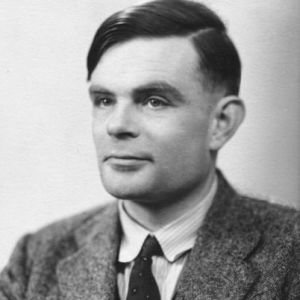
\includegraphics[width=0.5\textwidth]{img/turing-portrait.jpg}
  \caption{Turing would be proud}
  \label{fig:turing}
\end{figure}

\section{Results} %TODO update section

P was shown to equal NP, as NP has been shown to equal P.

\section{Discussion} %TODO update section

Wow.

\printbibliography


\end{document}